%%%%%%%%%%%%%%%%%%%%%%%%%%%%%%%%%%%%%%%%%%%%%%%%%%%%%%%%%%%%%%%%%%%%%%%%%%%%%%%%
%2345678901234567890123456789012345678901234567890123456789012345678901234567890
%        1         2         3         4         5         6         7         8

% \documentclass[letterpaper, 10 pt, conference]{ieeeconf}  % Comment this line out if you need a4paper

\documentclass{amsart}
\usepackage[T1]{fontenc}
% \usepackage[margin=1.25in]{geometry}

%\documentclass[a4paper, 10pt, conference]{ieeeconf}      % Use this line for a4 paper

% \IEEEoverridecommandlockouts                              % This command is only needed if 
%                                                           % you want to use the \thanks command

% \overrideIEEEmargins                                      % Needed to meet printer requirements.

%In case you encounter the following error:
%Error 1010 The PDF file may be corrupt (unable to open PDF file) OR
%Error 1000 An error occurred while parsing a contents stream. Unable to analyze the PDF file.
%This is a known problem with pdfLaTeX conversion filter. The file cannot be opened with acrobat reader
%Please use one of the alternatives below to circumvent this error by uncommenting one or the other
%\pdfobjcompresslevel=0
%\pdfminorversion=4

% See the \addtolength command later in the file to balance the column lengths
% on the last page of the document

% The following packages can be found on http:\\www.ctan.org
%\usepackage{graphics} % for pdf, bitmapped graphics files
%\usepackage{epsfig} % for postscript graphics files
%\usepackage{mathptmx} % assumes new font selection scheme installed
%\usepackage{times} % assumes new font selection scheme installed
%\usepackage{amsmath} % assumes amsmath package installed
%\usepackage{amssymb}  % assumes amsmath package installed
\usepackage{cite}
\usepackage{amsmath,amssymb,amsfonts,mathtools}
\usepackage[ruled, lined, commentsnumbered, longend]{algorithm2e}
% \usepackage{algorithmic}
\usepackage{algpseudocode}
\usepackage{graphicx}
\usepackage{textcomp}
\usepackage{xcolor}
\usepackage{balance}
% \usepackage[backend=bibtex,bibstyle=ieee,citestyle=numeric-comp]{biblatex}

\DeclareMathOperator*{\argmin}{argmin}
\DeclareMathOperator*{\argmax}{argmax}
\DeclareMathOperator*{\argminB}{argmin}

\title{\LARGE \bf
Bayesian directed sampling for efficient local model validation
}

\author{Kellan Moorse and Richard Murray}

% \author{\IEEEauthorblockN{Kellan Moorse}
% \IEEEauthorblockA{\textit{California Institute of Technology} \\
% Pasadena, United States \\
% kmoorse@caltech.edu}


% \author{Kellan Moorse$^{1}$ and Richard Murray$^{2}$% <-this % stops a space

% % \thanks{$^{1}$K. Moorse is a graduate student at California Institute of Technology,
% % Pasadena, USA
% %         {\tt\small kmoorse@caltech.edu}}%
% % \thanks{$^{2}$Richard Murray is with the Department of Control and Dynamical Systems, California Institute of Technology,
% % Pasadena, USA
% %         {\tt\small murray@cds.caltech.edu}}%
% % \thanks{We acknowledge funding from AFOSR Test and Evaluation Program, grant FA9550-19-1-0302}% <-this % stops a space
% % \date{}
% }



\begin{document}



\maketitle
\thispagestyle{empty}
\pagestyle{empty}


%%%%%%%%%%%%%%%%%%%%%%%%%%%%%%%%%%%%%%%%%%%%%%%%%%%%%%%%%%%%%%%%%%%%%%%%%%%%%%%%
\begin{abstract}

Classification problems are typically characterized by categorical data points, but real world data is often continuous, being truncated to discrete categories for the purpose of conforming to standard methods. We propose a method for exploiting the additional information of real-valued data to efficiently train a classifier. In particular, we consider the problem of estimating the subset of test conditions under which a simplified model---or set of simplified models---accurately approximates the behavior of a true system. We approach the problem by proposing a compact set of possible test conditions, and an unknown but samplable continous validity function over that set that quantifies the accuracy of the model under each possible condition. We propose a novel Bayes estimator that optimally directs function sampling to greedily minimize the expected posterior misclassification rate of the valid set, which we call minimum posterior misclassification sampling (GP-MPM), and we show that the the method can be extended to approximate the valid sets of a partially ordered set of models, with sample complexity growing sublinearly with the number of models. In empirical testing, we show that the algorithm's estimated valid set approaches the true valid set much more quickly than undirected sampling, even with small sample sizes.
\end{abstract}


%%%%%%%%%%%%%%%%%%%%%%%%%%%%%%%%%%%%%%%%%%%%%%%%%%%%%%%%%%%%%%%%%%%%%%%%%%%%%%%%
\section{Introduction}

As engineered systems like autonomous vehicles become more complex, it becomes increasingly necessary to rely on simulations to characterize a huge set of behaviors of interest, and while researchers often have access to extremely high-fidelity models that closely approximate system behavior \cite{mcruer75, pearce62}, these models are too costly to use for every test. And in many cases, the decision of when to dedicate the resources to use these highly detailed models, and when to settle for a simpler, cheaper one, is done heuristically. Simpified models may produce test results that are inconsistent with the behavior of the true system, and it is not always possible to analytically compute the conditions under which a simplified model diverges from the system's true behavior, so naively utilizing the results of a model carries a nontrivial risk of making erroneous conclusions about the true system behavior. However, we will demonstrate that even when model mismatch is not analytically computable, it is still possible to sample the model's performance relative to the true system behavior and make probabilistic statements about the magnitude of the mismatch.
\newline

Existing methods for quantifying model performance often treat it as a random variable drawn from a single univariate continuous probability distribution. By assuming a particular analytical distribution characterized by parameters, $\theta$, with cumulative distribution function, $F(x|\theta)$, a tester can sample the performance and infer the parameters of the distribution via any of a number of well-established methods, from classical maximum likelihood estimation \cite{gelman13}, to expectation-maximization \cite{dempster77}, to further specialized methods for specific distributions \cite{tang19,ren22}. And once we have an estimate of the parameters of a distribution, it is trivial to find probabilistic bounds on the values taken by its corresponding random variable $X$ directly from the definition of its cumulative distribution function $F(x|\theta)$

\begin{equation}
    F(x\,|\,\theta) = \mathbb{P}[X<x\,|\,\theta] \nonumber
\end{equation}

Further, it is generally possible to calculate confidence intervals on the parameter estimates produced by the above methods. This allows us to calculate bounds of the form

\begin{equation}
    \mathbb{P}[F(x)<\epsilon]<\gamma \nonumber
\end{equation}

In other words, we calculate a bounded probability $\gamma$ that a value drawn from the distribution of interest is smaller than $\epsilon$. This is useful because it accounts for both the measurement noise in sampling the system's performance, and our uncertainty in the parameters of the distribution being sampled. Further, we can calculate this kind of bound directly, without assuming any prior parametric distribution, via methods such as value-at-risk calculations \cite{jorion06,kuester06}. However, while the results of these methods are sound, and useful in a wide variety of applications, each one assumes that every observation of a system is drawn from a single univariate distribution, so they are incapable of capturing conditional properties. Many simplified models are designed to be conditionally valid---that is, they consistently perform well under some conditions, such as when a simplifying assumption holds, and consistently perform poorly when those conditions are not met. In order to capture and quantify these conditional properties, it is necessary to employ a more sophisticated model.
\newline

Rather than dealing with parametric multivariate distributions, which can be handled similarly to their univariate counterparts, we consider the special case of a conditional distribution $p(x|\phi)$, where samples $x$ are drawn from different distributions depending on the conditions $\phi$ of the draw. For example, performance values for a linearized dynamical model will be drawn from a distribution with a higher mean if the system is near the fixed point of the linearization. This model allows us to efficiently sample the function to infer attibutes like the locations of its optima, with \cite{chowdhury17}\cite{srinivas09} or without \cite{bonyadi17}\cite{akella22} assuming an underlying parametric distribution. But optimum-finding algorithms do a poor job of characterizing the function away from a single point, and global sampling, such as a grid search, has the opposite problem of collecting unnecessary samples and becoming intractably sample-intensive in higher dimensions \cite{chen15}\cite{he20}.

Rather than searching for a single optimum, or characterizing an entire high-dimensional function, we present a method for estimating the subset of the condition space over which the distribution $p(x|\phi)$ takes values $x>0$ with arbitrary confidence. As we show below, carefully chosen definitions produce a distribution where this positive set is identically the set under which our model of interest is valid. While many data-driven methods exist for estimating subsets \cite{ahmed03} \cite{boser92}\cite{gibbs00}, many assume that sampling only produces discrete categorical data, and none of them provide an algorithm for efficient directed sampling, instead relying on large quatities of data to refine the estimated subset. Below, we present a method for highly efficient directed sampling for the estimation of the positive subset of an unknown validity function. We further extend this algorithm to partially-ordered sets of models, generating a validity map that reports, for any given test condition, the lowest-order model that is still a good approximation of the true system, with arbitrary confidence.

\section{Definitions}
\noindent\textbf{Validity Metric.} We begin by formalizing the conditions under which a model may be tested. Let $\Phi$ be a compact set in $\mathbb{R}^p$, where a vector $\phi\in\Phi$ is the set of conditions describing a given test---such as obstacle locations, road friction conditions, etc.---and let $v:\Phi\rightarrow\mathbb{R}$ be a continuous function which maps test conditions onto a scalar validity metric. This validity function is the function we seek to estimate, and it is assumed to exist for all $\phi\in\Phi$. While its values are unknown initially, its value can be sampled for any $\phi\in\Phi$.

To facilitate the later extension to multiple models, we define a pair of intermediate functions $[m^i:\Phi\rightarrow\mathbb{R}^q]_{i\in\{0,1\}}$ which map test conditions onto a vector of observations from model $i$. We also give a formulation of the validity function which is an explicit pairwise comparison between the observations from two models.

\begin{equation}
    v^{01}(\phi) = v(m^0(\phi), m^1(\phi))
    \label{eq:valorig}
\end{equation}
\smallskip

One possible instantiation of this framework is that $m^0(\phi)$ and $m^1(\phi)$ correspond to traces of the position of the center of mass of an autonomous agent performing a task under some condition $\phi$ in experiment and in simulation, respectively. Then $v^{01}(\phi)$ may be the maximum norm difference between those position traces over the course of the task

\begin{align}
\begin{split}
    m^0(\phi)&=[x^0_1,...x^0_T] \\
    m^1(\phi)&=[x^1_1,...x^1_T] \\
    v^{01}(\phi) &= \max\limits_{t\in\{1...T\}} \|x^0_t-x^1_t\|
\end{split}
\end{align}
\smallskip

In the following analysis, we use $v(\phi)$ as shorthand for $v^{01}(\phi)$, where model $0$ is the true system, and model $1$ is the simplified model of interest.

and it is initially unknown, but its value can be sampled for any $\phi$. We define the model to be valid when $v(\phi)>0$, and it follows that the valid set, or the set of $\phi$ for which the model is valid, is

\begin{equation}
    V=\{\phi\in\Phi\ |\ v(\phi)>0\}
\end{equation}

By this definition, the problem of set estimation is transformed into a problem of function estimation.

The validity function is sampled by running the same test on both a simplified model and the ground The function of interest $v(\phi)$ is continuous but otherwise unconstrained, which makes Gaussian process regression a strong method for estimation. 
\linebreak

%##########################################################
%########   Gaussian Process Definition
%##########################################################
\noindent\textbf{Gaussian Process Regression.} We propose Gaussian processes as a model for estimating $v(\phi)$ for two reasons: first, complex engineering systems are often comprised of many interacting subsystems that each contribute to measurements of the system's properties. By the central limit theorem, uncertainty in those measurements is likely to be well-modeled by a Gaussian distribution. And second, real physical systems are generally continuous---i.e. small changes to their inputs result in small changes to their outputs. The Gaussian process model assumes these two properties, but no other structure in the function being approximated, so we can make good approximations of a wide variety of functions.

Let $GP_\Phi(\mu(\cdot),k(\cdot,\cdot))$ be a Gaussian process, representing a set of random variables $[g(\phi)]_{\phi\in\Phi}$, such that each finite subset $[g(\phi)]_{i=1}^k$ is jointly Gaussian with mean and covariance

\begin{equation}
    \mathbb{E}[(g(\phi_i)] = \mu(\phi_i)
    \label{eq:jointmean}
\end{equation}

\begin{multline}
    \mathbb{E}[(g(\phi_i)-\mu(\phi_i))(g(\phi_j)-\mu(\phi_j))]=k(\phi_i,\phi_j) \\
    1\leq i,j\leq m,\ m\in \mathbb{N}
    \label{eq:jointcov}
\end{multline}
\smallskip

We use the prior $GP_\Phi(0,k(\cdot,\cdot))$, with mean zero and variance one, but the prior variance can be scaled to any positive value without loss of generality. Further, we use a typical squared exponential kernel

\begin{equation}
    k(\phi,\phi') = exp\bigg(\frac{\|\phi-\phi'\|_2}{2l^2}\bigg)
\end{equation}

where $l$ is a hyperparameter corresponding to the scale of the exponential. It is possible---and in many cases desireable---to estimate the hyperparameters of a Gaussian process to optimize its regression (\cite{blum13,chen16}), but this requires additional samples of the function, which we have assumed is the rate-limiting step of our algorithm. So for simplicity, we set $l$ as a constant at the beginning of the procedure. We also assume normally-distributed measurement noise $\epsilon_t\sim\mathcal{N}(0,\lambda)$ added to each sample, where $\lambda$ is also set as a hyperparameter.

Given a set of sample locations $A_t=(\phi_1,...,\phi_t)$, we call the corresponding set of observed rewards $v_{1:t}=[v_1,...,v_t]^T$. Then we define the kernel matrix and kernel vector

\begin{align}
\begin{split}
    K_t &= [k(\phi,\phi')]_{\phi,\phi'\in A_t} \\
    k_t(\phi) &= [k(\phi_1,\phi),...,k(\phi_t,\phi)]^T
\end{split}
\end{align}
\smallskip

The observed reward vector and the true function $f(\phi)$ are then jointy Gaussian given $A_t$

\begin{equation}
    \begin{bmatrix}
        f(\phi)\\
        v_{1:t}
    \end{bmatrix}
    \sim\mathcal{N}\Bigg(0,
    \begin{bmatrix}
        k(\phi,\phi) & k_t(\phi)^T \\
        k_t(\phi) & K_t+\lambda I
    \end{bmatrix}
    \Bigg)
\end{equation}
\smallskip

and the posterior distribution over $f$ is $GP_\Phi(\mu_t(\cdot),k_t(\cdot,\cdot))$, where

\begin{flalign}
    \small
    \mu_t(\phi) =& k_t(\phi)^T (K_t+\lambda I)^{-1} v_{1:t} \label{eq:gpmean} \\
    k_t(\phi,\phi') =& k(\phi,\phi') \nonumber \\
    &-k_t(\phi)^T(K_t+\lambda I)^{-1}k_t(\phi') \label{eq:gpk} \\ 
    \sigma_t^2(\phi) =& k_t(\phi,\phi) \label{eq:gpvar}
\end{flalign}
\smallskip

\section{Sampling Method}

\noindent\textbf{Efficient Posterior Sampling.} In order to define a Bayes estimator, we need a computationally efficient representation of the posterior distribution. Below, we derive a recursive definition of the Gaussian process posterior.

Note that in \eqref{eq:gpmean}, omitting the last data point $x_t$ is equaivalent to removing the last elements of $k_t(\phi)$ and $v_{1:t}$, and removing the last row and column from $K_t$


\begin{align}
\begin{split}
    k_t(\phi)^T &= 
    \begin{bmatrix}
        k(\phi_1,\phi)&\hdots&k(\phi_t,\phi)
    \end{bmatrix}
    \\
    k_{t-1}(\phi)^T &= 
    \begin{bmatrix}
        k(\phi_1,\phi)&\hdots&k(\phi_{t-1},\phi)
    \end{bmatrix}
    \label{eq:tstepk}
\end{split}
\end{align}

\begin{align}
\begin{split}
    K_t+\lambda I &= 
    \begin{bmatrix}
        k(\phi_1,\phi_1)&\hdots&k(\phi_1,\phi_t) \\
        \vdots & \ddots & \vdots \\
        k(\phi_t,\phi_1)&\hdots&k(\phi_t,\phi_t)
    \end{bmatrix}
    \\
    K_{t-1}+\lambda I &= 
    \begin{bmatrix}
        k(\phi_1,\phi_1)&\hdots&k(\phi_1,\phi_{t-1}) \\
        \vdots & \ddots & \vdots \\
        k(\phi_{t-1},\phi_1)&\hdots&k(\phi_{t-1},\phi_{t-1})
    \end{bmatrix}
    \label{eq:tstepK}
\end{split}
\end{align}

\begin{equation}
    v_{1:t} = 
    \begin{bmatrix}
        v_1 \\
        \vdots \\
        v_t
    \end{bmatrix}
    ,\ 
    v_{1:t-1} = 
    \begin{bmatrix}
        v_1 \\
        \vdots \\
        v_{t-1}
    \end{bmatrix}
    \label{eq:tstepv}
\end{equation}
\smallskip

Using \eqref{eq:tstepk}-\eqref{eq:tstepv}, and noting that $k(\phi,\phi)=1$ for any $\phi$, we can write each term of \eqref{eq:gpmean} at time $t$ in terms of its expression at time $t-1$

\begin{equation}
    k_t(\phi)^T=
    \begin{bmatrix}
        k_{t-1}(\phi)^T, k(\phi_t,\phi)
    \end{bmatrix}
\end{equation}

\begin{align}
\begin{split}
    K_t &=
    \begin{bmatrix}
        K_{t-1} & k_{t-1}(\phi_t) \\
        k_{t-1}(\phi_t)^T & 1
    \end{bmatrix}
    \\
    K_t+\lambda I &=
    \begin{bmatrix}
        K_{t-1}+\lambda I & k_{t-1}(\phi_t) \\
        k_{t-1}(\phi_t)^T & 1 + \lambda
    \end{bmatrix}
\end{split}
\end{align}

\begin{equation}
    v_t = 
    \begin{bmatrix}
        v_{t-1} \\
        v_t
    \end{bmatrix}
\end{equation}
\smallskip

Labeling the block components of $K_t+\lambda I$, we can rewrite \eqref{eq:gpmean} as

\begin{equation}
    \mu_t(\phi) =
    \begin{bmatrix}
        k_{t-1}(\phi)^T & k(\phi_t,\phi)
    \end{bmatrix}
    R^{-1}
    \begin{bmatrix}
        v_{1:t-1} \\
        v_t
    \end{bmatrix}
    \label{eq:gpmeanblock}
\end{equation}

\begin{align}
    R&=
    \begin{bmatrix}
        A & B \\
        B^T & D
    \end{bmatrix}
    \nonumber \\
    A &= K_{t-1}+\lambda I \nonumber \\
    B &= k_{t-1}(\phi) \nonumber \\
    D &= 1+\lambda \nonumber
\end{align}
\smallskip
And we note several useful definitions that follow from the block form of R

\begin{align}
    \mu_{t-1}(\phi) &= k_{t-1}(x)^T A^{-1} v_{1:t-1} \label{eq:blockdefmu}\\ 
    \frac{1}{\sigma_{t-1}^2(\phi_t)+\lambda} &= (D-B^T A^{-1}B)^{-1} \label{eq:blockdefsig}
\end{align}
\smallskip

Because the block matrix is Hermitian, its inverse is given in \cite{lu02} to be

\begin{equation}
    \begin{bmatrix}
        A & B \\
        B^T & D
    \end{bmatrix}^{-1}
    =
    \begin{bmatrix}
        E & F \\
        G & H
    \end{bmatrix}
    \label{eq:blockinverse}
\end{equation}

\begin{align}
    E &= A^{-1}+A^{-1}B(D-B^T A^{-1} B)^{-1}B^T A^{-1} \nonumber \\
    F &= -A^{-1}B(D-B^T A^{-1} B)^{-1} \nonumber \\
    G &= -(D-B^T A^{-1} B)^{-1}B^T A^{-1} \nonumber \\
    H &= (D-B^T A^{-1} B)^{-1} \nonumber
\end{align}
\smallskip

Substituting \eqref{eq:blockinverse} into \eqref{eq:gpmeanblock} and multiplying out the matrices, we find a computable expression for the posterior mean $\mu(\phi)$ as a function of the prior distribution and a newly collected data point $(\phi_t,v_t)$

\begin{align}
\begin{split}
    \tiny
    \mu&(\phi) = k_{t-1}(\phi)^T A^{-1} v_{1:t-1} \\
    &+ k_{t-1}(\phi)^T A^{-1} B (D-B^T A^{-1} B)^{-1} B^T A^{-1} v_{1:t-1} \\
    &- k(\phi,\phi_t)(D-B^T A^{-1} B)^{-1} B^T A v_{1:t-1} \\
    &- k_{t-1}(\phi)^T A^{-1} B(D-B^T A^{-1}B)^{-1}v_t \\
    &+ k_(\phi,\phi_t)(D-B^T A^{-1}B)v_t
\end{split}
\end{align}

Combining like terms and using \eqref{eq:blockdefmu} and \eqref{eq:blockdefsig} to convert back from block matrix to GP parameters, we arrive at a much simpler form

\begin{equation}
    \mu_t(\phi,\phi_t,v_t) = \mu_{t-1}(\phi) + \frac{k_{t-1}(\phi,\phi_t)}{\sigma_{t-1}^2(\phi_t)+\lambda}(v_t-\mu_{t-1}(\phi_t))
    \label{eq:recmu}
\end{equation}

Following an identical procedure but starting from \eqref{eq:gpvar}, we also derive a recursive expression for the variance

\begin{equation}
    \sigma_t^2(\phi,\phi_t) = \frac{\lambda k_{t-1}(\phi,\phi_t)}{\sigma_{t-1}^2(\phi_t)+\lambda}
    \label{eq:recsig}
\end{equation}
\smallskip

\noindent\textbf{Bayes Estimator.} Having derived conscise definitions for the posterior mean and variance of the Gaussian process, we propose a novel Bayes estimator which minimizes the expected posterior misclassification rate. Let $P^m_t(\phi)$ be the misclassification error rate at $\phi$: the probability that the true function value $f(\phi)$ has a different sign than the posterior Gaussian process mean after t samples


\begin{equation}
    P^e_t (\phi) = \mathbb{P}[\text{sgn}\,f(\phi)\neq \text{sgn}\,\mu_t(\phi)]
\end{equation}

From the Gaussian cumulative distribution function, this is equal to:

\begin{equation}
    P^e_t(\phi) = \frac{1}{2}\text{erfc}\bigg(\frac{|\mu_t(\phi)|}{\sqrt{2}\sigma_t(\phi)}\bigg)
\end{equation}
\smallskip

Now let $Z_{t-1}(\phi_t)\sim\mathcal{N}(\mu_{t-1}(\phi_t),\sigma_{t-1}(\phi_t))$ be a random variable corresponding to value observed upon sampling at $\phi_t$, conditioned on the previously observed values $(A_{t-1},v_{1:t-1})$. Then $P_t^e(\phi,\phi_t,Z_{t-1}(\phi_t))$ is the posterior misclassification error at $\phi$, and its expectation is

\begin{equation}
    \small
    \mathbb{E}_{z}[P_t^e(\phi,\phi_t,Z_{t-1}(\phi_t)] = \frac{1}{2}\text{erfc}\bigg(\frac{|\mu_t(\phi,\phi_t,Z_{t-1}(\phi_t)|}{\sigma_t^2(\phi,\phi_t)}\bigg)
    \label{eq:exprec}
\end{equation}
\smallskip

We define the global misclassification rate as the expectation of the local misclassification rate across all $\phi\in\Phi$---that is, the probability of drawing a misclassified $\phi$ from a uniform distribution over $\Phi$

\begin{equation}
    g(\phi_t) = \frac{\int_\Phi \mathbb{E}_{z}[P_t^e(\phi,\phi_t,Z_{t-1}(\phi_t))] d\phi^{(1)}...d\phi^d\phi^{(p)}}{\int_\Phi d\phi^{(1)}...d\phi^d\phi^{(p)}}
    \label{eq:objfull}
\end{equation}
\smallskip

The minimizer of $g(\phi_t)$ is, by definition, the point that minimizes the expected posterior global misclassification rate. However, the function $P_t^e(\phi,\phi_t,Z_{t-1}(\phi_t))$ has no assumed structure in $\phi$ beyond continuity, and numerically computing the nested integral over all $\phi\in\Phi$ and all $Z_{t-1}(\phi_t)\in\mathbb{R}$ is computationally expensive even in low dimensions---and prohibitively so in higher dimensions. So we implement a pair of approximations to make the computation tractable.

First, we consider the expectation over $P_t^e(\phi,\phi_t,Z_{t-1}(\phi_t))$. Because $Z_{t-1}(\phi_t)$ takes any real-numbered value, the expectation is given by:

\begin{equation}
    \int_\mathbb{R}p(z)P_t^e(\phi,\phi_t,z)dz
\end{equation}
\smallskip

where $p(z)$ is the probability density function over realizations $z$ of $Z_{t-1}(\phi_t)$. We note that the expectation of a function of a gaussian random variable is equal to the function value at the mean of the random variable if (but not only if) the function is linear

\begin{align}
    y(x)&=x \nonumber \\
    p(x)&= \frac{1}{\sigma \sqrt{2\pi}}\,exp\Big(-\frac{1}{2}\big(\frac{x-\mu}{\sigma}\big)^2\Big)\nonumber \\
    \mathbb{E}[y(x)]& = \int_\mathbb{R}p(x)y(x)dx = y(\mu)
\end{align}
\smallskip

Equation \eqref{eq:recmu} shows that $\mu_t(\phi)$ depends linearly on $Z_{t-1}(\phi_t)$, \eqref{eq:exprec} shows that the argument of erfc depends linearly on $\mu_t(\phi)$ except precisely at zero, and the erfc function itself is smooth, approaching linearity as the absolute value of its argument gets large. So, if we replace $\mathbb{E}_{z}[P_t^e(\phi,\phi_t,Z_{t-1}(\phi_t))]$ with $P_t^e(\phi,\phi_t,\mu_{t-1}(\phi_t))$, the approximation is very good for large $|\mu_t|/\sigma_t$. The negative discontinuity in the derivative of $\text{erfc}(|\cdot|)$ at zero means that we slightly underestimate $P_t^e$ at small $|\mu_t|/\sigma_t$, but because the Bayes estimator only considers relative values of the loss function, this has a minimal effect on its chosen actions.

Because we now assume that, in expectation, each newly collected sample at $\phi_t$ lands on $\mu_{t-1}(\phi_t)$, the difference term in \eqref{eq:recmu} is identically zero and $\mu_{t-1}(\phi)=\mu_t(\phi)$ for all $\phi\in\Phi$. So there is no need to calculate the expected posterior mean $\mathbb{E}_z[\mu_t(\phi)]$, reducing the computation time of the expectation calculation by roughly half.

Second, we note that for our chosen kernel function $k(\phi,\phi')=exp(\|\phi-\phi'\|_2/2l^2)$, the covariance asyptotically approaches zero as the distance between the points grows large

\begin{align}
    \lim_{s\rightarrow\infty} |\sigma_t^2(\phi)-\sigma_t^2(\phi')|=0 \\
    s = \|\phi-\phi'\|_2 \nonumber
\end{align}

The squared-exponential has particularly light tails, so the covariance can be treated as negligible for any points more than a small number of scale-lengths apart. This means that instead of integrating the expected posterior misclassification over all of $\Phi$, we can integrate only over a $p$-ball around $\phi_t$, with radius $\alpha l$. $\alpha$ is left as a hyperparameter of the method, but $\alpha=2$ is a reasonable choice for low-dimensional problems, capturing 95\% of the kernel's mass in the one-dimensional case. In higher dimensions, the same $\alpha$ captures a smaller proportion of the kernel's mass, so it may be necessary to choose a larger value.

Incorporating these approximations, and omitting the denominator of \eqref{eq:objfull} which does not depend on $\phi_t$ and only acts as a normalizing factor, we arrive at a simplified loss function whose optimizer closely approximates that of the true Bayes estimator

\begin{align}
    \label{eq:objapprox}
    \tilde{g}(\phi_t)=\int_B P_t^e(\phi,\phi_t,\mu_{t-1}(\phi_t))d\phi^{(1)}...d\phi^{(p)} \\
    B = \{\phi\in\Phi\ |\ \|\phi-\phi_t\|_2<\alpha l\} \nonumber
\end{align}

Because this loss function is fast to compute, we can apply it iteratively to estimate the valid set of a function. However, the optimum is undefined for the prior $GP(0,k)$, so it must be initalized with at least one sample collected using a different method. In practice, the initialization is a small set of $t_0$ points drawn from a uniform distribution over $\Phi$. The full procedure is shown in alg. \ref{mpmsingle}.

\begin{algorithm}
    \small
    \label{mpmsingle}
    \caption{GP-MPM: Single Model}
    \textbf{Input}: Prior GP(0,k), parameters $\lambda,\alpha,t_0$\\
    Set $A_{t_0} = [\phi_j \sim U(\Phi)]_{j=1}^{t_0}, v_{1:t_0}=[f(\phi_j)+\epsilon_j]_{j=1}^{t_0} $\\
    \For{t=1,2,3...T}{
        Choose $\phi_t = \argmin\limits_{\phi\in\Phi}  \int_B P_t^e(\phi,\phi_t,\mu_{t-1}(\phi_t))d\phi^1...d\phi^p$ \\
        \Indp where $B = \{\phi\in\Phi\ |\ \|\phi-\phi_t\|_2<\alpha l\}$ \\
        \Indm Observe validity $v_t = f(\phi_t)+\epsilon_t$ \\
        Perform update to get $\mu_t$ and $\sigma_t$ using \eqref{eq:gpmean}--\eqref{eq:gpvar}
    }
\end{algorithm}

\section{Model Sets}

From the approximate Bayes estimator in \eqref{eq:objapprox}, it is possible to extend the method to estimate valid sets for a set of models. Let $M=\{m^i\}_{i=0}^n$ be a finite set of models, each of which is a function mapping conditions to measurements

\begin{equation}
    [m^i:\Phi\rightarrow\mathbb{R}^q]_{i=0}^n\\
\end{equation}

and we generalize the intermediate function in \eqref{eq:valorig} to map measurements from any two models onto a scalar validity metric

\begin{equation}
    v^{ij}(\phi) = \tilde{v}(m^i(\phi),m^j(\phi))
\end{equation}

Because models are always compared against the true system behavior $m^0(\phi)$, we define the shorthand $v^j(\phi)=v^{0j}(\phi$), and following the convention of the single-model case

\begin{equation}
    V^i = \{\phi\in\Phi\ |\ v^i(\phi)>0\}
\end{equation}

We then assume that the set of models can be organized into a partial order, where a model being greater in the order means that its validity is greater under all conditions

\begin{equation}
    m^i>m^j\iff v^i(\phi)>v^j(\phi)\ \forall\phi\in\Phi
\end{equation}

This futher implies that the valid set for a given model is a superset of the valid set of each lesser model in the order

\begin{equation}
    m^i>v^j\implies \bigcap_{i|m^i>m^j} V^i \supset V^j
\end{equation}

\begin{algorithm*}
    \caption{GP-MPM: Model Set}
    \textbf{Input}: Priors $[GP_i(0,k)]_{i=1}^n$, parameters $\lambda,\alpha,t_0$\\
    Set $A_{t_0} = [\phi_i \sim U(\Phi)]_{i=1}^{t_0}, [v^j_{1:t_0}=[f(\phi_i)+\epsilon_i]_{i=1}^{t_0}]_{j=1}^n $\\
    \For{i=1,2,3...n}{
        \For{t=1,2,3...T}{
            Choose $\phi_t = \argmin\limits_{\phi\in\Phi}  \int_B P_t^e(\phi,\phi_t,\mu^j_{t-1}(\phi_t))d\phi^1...d\phi^p$ \\
            Observe validities $[v^j_t = f^j(\phi_t)+\epsilon_t]_{j\leq i}$ \\
            Perform updates to get $[\mu^j_t]_{j\leq i}$ and $[\sigma^j_t]_{j\leq i}$ using \eqref{eq:gpmean}--\eqref{eq:gpvar}
        }
    }
\end{algorithm*}

\begin{figure}[htbp]
    \centerline{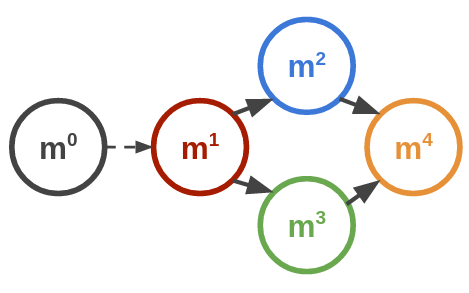
\includegraphics[width=0.9\columnwidth]{img/model_tree3.png}}
    \caption{An example model graph with a nontrivial order, asserting that each model performs better than the model(s) below it.}
    \label{fig:modeltree}
\end{figure}

\begin{figure}[htbp]
    \centerline{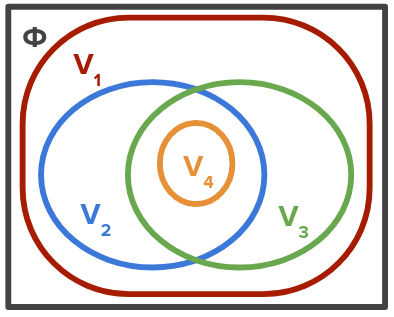
\includegraphics[width=0.9\columnwidth]{img/v_map.png}}
    \caption{A possible validity map corresponding to the ordered graph in Fig. \ref{fig:modeltree}. Note that each model's valid set is a subset of the valid sets of any models above it in the order.}
    \label{fig:vmap}
\end{figure}

\begin{figure}[htbp]
    \centerline{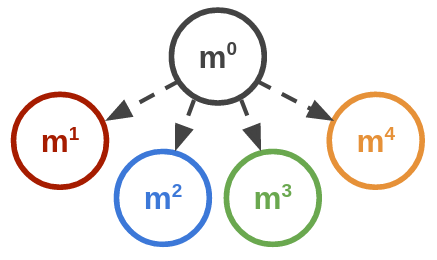
\includegraphics[width=0.9\columnwidth]{img/model_tree_unordered.png}}
    \caption{An example model graph with a trivial order that makes no assumptions about the relative performance of its models
    }
    \label{fig:modeltree2}
\end{figure}

The benefits of treating the models as a set are twofold: first, the rate-limiting step of the procedure is measuring the performance of the true system $m^0$, and if we have multiple models, we can re-use those measurements. Consider a pair of samples, $v^i(\phi^*)$ and $v^j(\phi^*)$. The former requires a measurement of $m^i(\phi^*)$ and the latter requires a measurement of $m^j(\phi^*)$, but both require a measurement of $m^0(\phi^*)$. In practice, the algorithm-directed measurements for one model can be repurposed to make undirected measurements for each other model, providing a preliminary dataset to initialize the directed sampling of models beyond the first.

Second, we can use the partial order to choose which valid sets to characterize first. Because the valid sets of lesser models are subsets of those of greater models, once we compute the valid set of a greater model $V^i$, we can exclude its complement from the search space for the valid set of a lesser model $V^j$---because we know that $v^j(\phi)$ is negative outside of $V^i$. In other words, instead of estimating $V^j$ as a subset of $\Phi$, we can estimate $V^j$ as a subset of $V^i$.

Fig. \ref{fig:modeltree} shows an example of an informative order, which can be used to direct sampling, and Fig. \ref{fig:vmap} shows a possible map of valid sets corresponding to that tree.

It is not necessary, however, to assume a strong order on the models. We can choose to assume only that the models $[m^1,...,m^n]$ are all less than $m^0$, as shown in Fig. \ref{fig:modeltree2}. This maximizes generality, but sacrifices the sampling efficiency gained by iteratively constricting the search space.

\section{Experiments}

To demonstrate the performance of the method, we construct several simple two-dimensional validity functions. For each function, we provide five points drawn from a uniform random distribution for initialization, and then iteratively choose additional points via GP-MPM until 100 total points have been sampled. For comparison, we also train several traditional classifiers on the same validity functions. For the support vector machine, we train the classifier on points chosen from a uniform random distribution. The continuous samples of the validity function are binarized by their signs. For the Gaussian process regressor, we train on a uniformly-spaced grid of points, and binarize the Gaussian process mean to produce a classifier.

in Fig. \ref{fig:multicomp}, we show that for all three example functions, GP-MPM dramatically outperforms both undirected classifers, consistently reaching an error rate of 0.1\% in less than 50 samples.

\begin{figure*}[htbp]
    \centerline{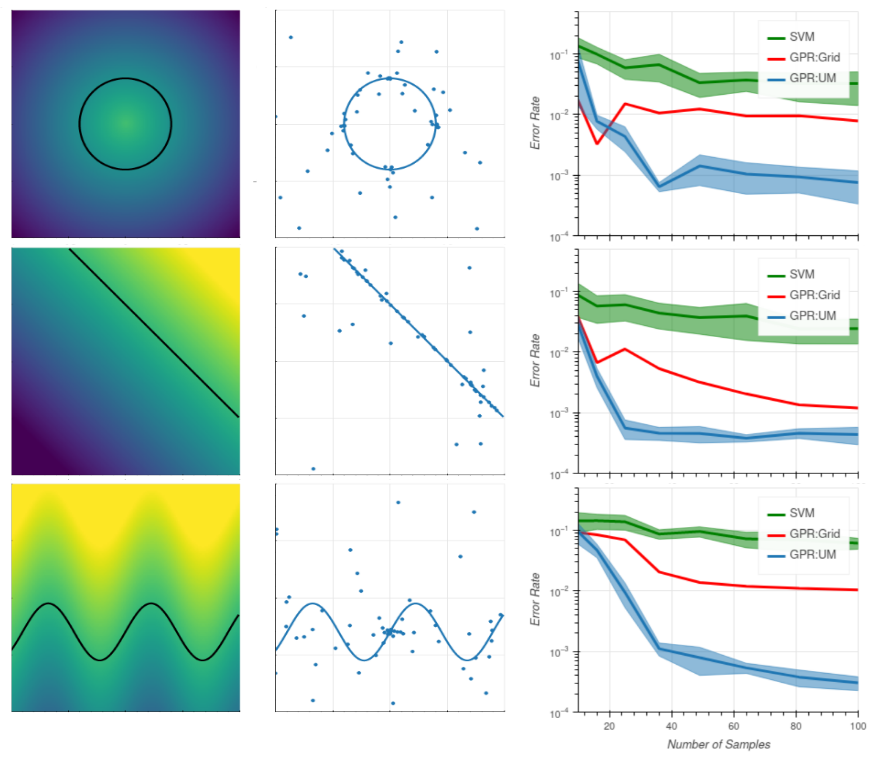
\includegraphics[width=\textwidth]{img/multi_comp.png}}
    \caption{Results of the GP-MPM algorithm for several known validity functions. Left: a heatmap of each validity function, with yellow corresponding to positive values, blue to negative, and the black line corresponding to $v(\phi)=0$. Center: the algorithm's estimate of each valid set with n=64. Right: global error rate for several classification methods as a function of the number of samples collected.}
    \label{fig:multicomp}
\end{figure*}

For a more grounded example, we also construct a simple double integrator dynamical system, and synthesize two controllers to reach a goal state while avoiding a circular obstacle. The first controller has knowledge of a true control barrier function, which is positive while safely avoiding the obstacle and negative while colliding. The second controller calculates the control barrier function from a simplified single integrator approximation of the true dynamics. In Fig. \ref{fig:expdemo}, we show an example case where the first controller (green) successfully avoids the obstacle, while the second controller (blue) collides.

\begin{figure}[htbp]
        \centerline{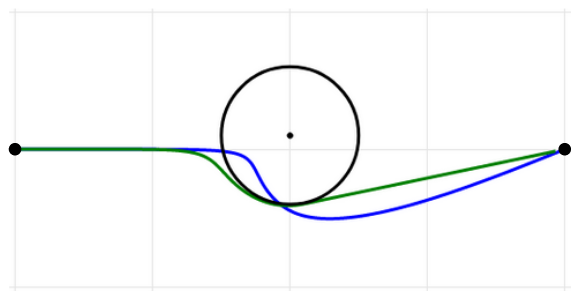
\includegraphics[width=0.9\columnwidth]{img/exp_demo.png}}
        \caption{An example pair of paths generated by two controllers synthesized for a double integrator system to reach a goal while avoiding a circular obstacle. In green, the controller enforces a control barrier function based on the true dynamics, and in blue, the controller enforces a control barrier function based on simplified single integrator dynamics. Initial position is (0,0) and the goal is at (0,4).}
        \label{fig:expdemo}
\end{figure}

\begin{figure}[htbp]
        \centerline{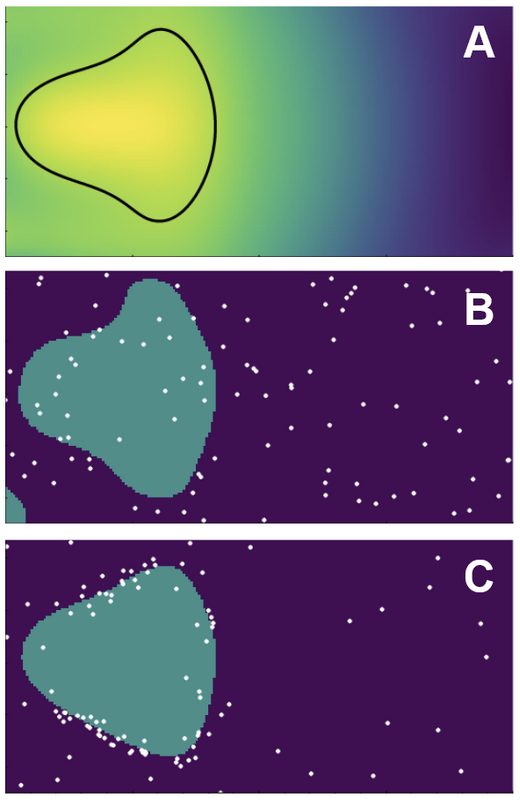
\includegraphics[width=0.9\columnwidth]{img/exp_result.png}}
        \caption{Results of the GP-MPM algorithm for exact and approximate synthesized safe controllers. (A) A gradient map representing the true validity function $v(\phi)$, with yellow representing negative values and dark blue positive. The black line denotes the boundary of the valid set $V$, with the enclosed region representing the complement of $V$. (B) The approximate valid set computed from a Gaussian process regression over uniform randomly chosen points. Dark blue represents the valid set, and sampled points are shown in white. (C) The approximate valid set computed by GP-MPM.}
        \label{fig:expres}
    \end{figure}

Using GP-MPM, then, we estimate the set of possible obstacle positions that result in a collision for the approximate controller (the exact controller is guaranteed not to collide \cite{molnar23}). We define $m^0$ and $m^1$ to be the exact and approximate models, respectively, the condition space to be a set of allowed $(x,y)$ positions for the obstacle $\Phi = (-0.5,0.5)\times(0,2)$, $y^0(\phi)$ and $y^1(\phi)$ as the position traces resulting from a particular obstacle position $\phi$, and $v(\phi)$ as the minimum value of control barrier function value for the approximate controller across a trace. In other words, when $v(\phi)$ is negative, obstacle position $\phi$ results in a collision for the approximate controller. In Fig. \ref{fig:expres} we show that in only 100 samples, GP-MPM produces a good approximation of the true valid set, which represents the set of obstacle positions that do not result in a collision for the optimal controller. GP-MPM reaches a misclassification rate of $0.9\%$, while uniform random sampling produces a poor approximation with a misclassification rate of $6.2\%$.

% To quantify the performance of the GP-MPM algorithm and compare it against alternative methods, we run a series of tests against known and directly samplable validity functions. For each test, we apply three methods of approximating the valid set:

% \begin{enumerate}
%     \item \textbf{GP-MPM} We draw five points from a uniform random distribution over $\Phi$ to initialize the Gaussian process, and then the algorithm runs unsupervised, with performance data collected at perfect square time steps, to match the grid search.
%     \item \textbf{Grid Search} We initialize a Gaussian process with the same kernel function as GP-MPM, but instead of directed sampling, the dataset consists of perfect square numbers of sample points, arranged in evenly-spaced grids.
%     \item \textbf{SVM} We binarize the validity function and sample it using uniform random draws from $\Phi$, using the resulting set of labels as training data for a support vector machine. The SVM uses a radial basis function with parameters chosen by an exponential grid search to maximize the classification rate.
% \end{enumerate}

% The results in fig. \ref{fig:multicomp} are striking, but perhaps unsurprising, as GP-MPM is able to exploit significantly more information about the validity function from each sample than either of the other methods. In every case, the GP-MPM algorithm reaches a 0.1\% misclassification rate with less than 50 function evaluations---and in one case as little as 25 samples. At 100 samples, it outperforms the undirected grid search by anywhere from a factor of 2 to a factor of 20, depending on the complexity of the valid set being approximated.

\section{Conclusion}

We have presented GP-MPM, a novel Bayes estimatorthat chooses actions to greedily minimize the expected posterior misclassification rate of a valid set by exploiting the continuous structure of the underlying validity function. In tests against known valid sets, GP-MPM significantly outperforms the misclassification rate of undirected grid-based sampling, especially at low sample sizes. The method has applications in any environment where running high-fidelity simulations is expensive, and the fidelity of low-cost alternatives is difficult or impossible to determine analytically.

\begin{thebibliography}{00}
\balance
\bibitem{ahmed03} M Ahmed, R Seraj, SMS Islam, ``The k-means algorithm: A comprehensive survey and performance evaluation,'' Electronics, 9(8), 1295, 2003
\bibitem{akella22} P Akella, A Dixit, M Ahmadi, JW Burdick, AD Ames, ``Sample-based bounds for coherent risk measures: Applications to policy synthesis and verification,'' arXiv:2204.09833, 2022 
\bibitem{blum13} M Blum, MA Riedmiller, ``Optimization of Gaussian process hyperparameters using Rprop,'' ESANN pp. 339-344, 2013
\bibitem{bonyadi17} MR Bonyadi, Z Michalewicz, ``Particle swarm optimization for single objective continuous space problems: a review,'' Evolutionary Computation. 25 (1): 1–54, 2017 
\bibitem{boser92} BE Boser, IM Guyon, VN Vapnik, ``A training algorithm for optimal margin classifiers,'' In Proceedings of the fifth annual workshop on Computational learning theory (pp. 144-152), 1992
\bibitem{chen15} S Chen, J Montgomery, A Bolufé-Röhler. 2015, ``Measuring the curse of dimensionality and its effects on particle swarm optimization and differential evolution,'' Appl. Intell. 42, 3 514–526, 2015
\bibitem{chen16} Z Chen, B Wang, ``How priors of initial hyperparameters affect Gaussian process regression models,'' arXiv:1605.07906, 2016
\bibitem{chowdhury17} SR Chowdhury, A Gopalan, ``On kernelized milti-armed bandits,'' Proceedings of the 34th International Conference on Machine Learning, PMLR 70:844-853, 2017
\bibitem{dempster77} AP Dempster, NM Laird, DB Rubin, ``Maximum Likelihood from Incomplete Data via the EM Algorithm,'' Journal of the Royal Statistical Society, Series B. 39 (1): 1–38, 1977
\bibitem{efron94} B Efron, RJ Tibshirani, \textit{An introduction to the bootstrap} CRC press, 1994
\bibitem{gelman13} A Gelman, JB Carlin, HS Stern, DB Dunson, A Vehtari, DB Rubin,\textit{Bayesian data analysis}, CRC press, 2013
\bibitem{gibbs00} MN Gibbs and DJC Mackay, ``Variational Gaussian process classifiers,'' in IEEE Transactions on Neural Networks, vol. 11, no. 6, pp. 1458-1464, 2000
\bibitem{he20} C He, S Huang, R Cheng, K Chen Tan, Y Jin, ``Evolutionary multiobjective optimization driven by generative adversarial networks (GANs),'' IEEE Trans. Cybern. (2020).
\bibitem{jorion06} P Jorion, ``Value at risk: the new benchmark for managing financial risk (3rd ed.),'' McGraw-Hill, 2006
\bibitem{kirschner21} J Kirschner, T Lattimore, C Vernade, C Szepesvari ``Asymptotically Optimal Information-Directed Sampling,'' Proceedings of Thirty Fourth Conference on Learning Theory, 134:2777-2821, 2021
\bibitem{kuester06} K Kuester, S Mittnik, M Paolella, ``Value-at-Risk Prediction: A Comparison of Alternative Strategies.'' Journal of Financial Econometrics. 4: 53–89, 2006
\bibitem{lu02} T Lu, S-H Shiou, ``Inverses of 2x2 block matrices,'' Comput Math Appl 43:119-129, 2002
\bibitem{mcruer75} DT McRuer, RH Klein, ``Automobile controllability -- driver/vehicle response for steering control volume I,'' Department of Transportation DOT-HS-359-3-762, 1975
\bibitem{nielsen12} F Nielsen, ``K-MLE: A fast algorithm for learning statistical mixture models'' IEEE International Conference on Acoustics, Speech and Signal Processing (ICASSP), 869–872, 2012
\bibitem{pearce62} BF Pearce, WA Johnson, RK Siskind, ``Analytical study of approximate longitudinal transfer functions for a flexible airframe,'' Air Force Systems Command Project 8219, Task 821901, 1962
\bibitem{ren22} T Ren, F Cui, S Sanghavi, N Ho, ``Beyond EM Algorithm on Over-specified Two-Component Location-Scale Gaussian Mixtures,'' arXiv preprint arXiv:2205.11078, 2022
\bibitem{srinivas09} N Srinivas, A Krause, SM Kakade, M Seeger, ``Gaussian process optimization in the bandit setting: No regret and experimental design,'' arXiv preprint arXiv:0912.3995, 2009
\bibitem{tang19} Y Tang, ``Beyond EM: A faster Bayesian linear regression algorithm without matrix inversions,'' Neurocomputing 378:435-440, 2019
\bibitem{molnar23} TG Molnar, AD Ames ``Safety-Critical Control with Bounded Inputs via Reduced Order Models,'' arXiv:2303.03247, 2023
\end{thebibliography}

\end{document}
